% !TeX root = ../RegT4.tex
% vim: ts=2 sw=2 spell:

\section{Idiot's section}

\begin{figure} \centering
    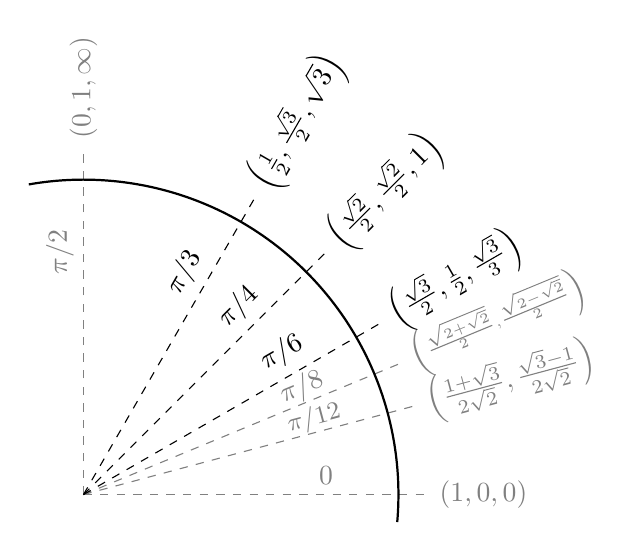
\begin{tikzpicture}[scale=4]
      \draw[gray,dashed] (0,0) --
      node[pos=.7, sloped, above] {\(0\)}
      node[pos=1, anchor=west, sloped] {\(\left(1,0,0\right)\)}
      (1.1,0);

      \draw[gray,dashed] (0,0) --
      node[pos=.7, sloped, above] {\(\pi/2\)}
      node[pos=1, anchor=west, sloped] {\(\left(0,1,\infty\right)\)}
      (0,1.1);

      \draw[gray,dashed] (0,0) --
      node[pos=.7, sloped, above = -3pt] {\small \(\pi/12\)}
      node[pos=1, anchor=west, sloped] {\(\left(\frac{1+ \sqrt3}{2\sqrt 2},\frac{\sqrt3 -1}{2\sqrt 2}\right)\)}
      ({1.1 *cos(15)}, {1.1 * sin(15)});

      \draw[gray,dashed] (0,0) --
      node[pos=.7, sloped, above = -3pt] {\(\pi/8\)}
      node[pos=1, anchor=west, sloped] {\(\scriptscriptstyle\left(\frac{\sqrt{2 + \sqrt{2}}}{2},\frac{\sqrt{2-\sqrt{2}}}{2}\right)\)}
      ({1.1 *cos(pi/8 r)}, {1.1 * sin(pi/8 r)});

      \draw[dashed] (0,0) --
      node[pos=.7, sloped, above] {\(\pi/6\)}
      node[pos=1, anchor=west, sloped] {\(\left(\frac{\sqrt 3}{2},\frac{1}{2},\frac{\sqrt3}{3}\right)\)}
      ({1.1 *cos(30)}, {1.1 * sin(30)});

      \draw[dashed] (0,0) --
      node[pos=.7, sloped, above] {\(\pi/4\)}
      node[pos=1, anchor=west, sloped] {\(\left(\frac{\sqrt 2}{2},\frac{\sqrt 2}{2}, 1\right)\)}
      ({1.1 *cos(45)}, {1.1 * sin(45)});

      \draw[dashed] (0,0) --
      node[pos=.7, sloped, above] {\(\pi/3\)}
      node[pos=1, anchor=west, sloped] {\(\left(\frac{1}{2},\frac{\sqrt 3}{2},\sqrt{3}\right)\)}
      ({1.1 *cos(60)}, {1.1 * sin(60)});

      \draw[black, thick] ({cos(-5)}, {sin(-5)}) arc (-5:100:1);
    \end{tikzpicture}
		\caption{
			Useful angles.
		}
\end{figure}

\begin{table} \centering
	\[
	\cos^2(x) + \sin^2(x) = 1 \quad \cosh^2(x) - \sinh^2(x) = 1
	\]
  \begin{tabular}{>{\(}l<{\)} @{\(\;=\;\)} >{\(}r<{\)}   >{\(}l<{\)} @{\(\;=\;\)} >{\(}r<{\)} }
    \toprule
    \cos(\alpha + 2\pi) & \cos(\alpha) & \sin(\alpha + 2\pi) & \sin(\alpha) \\
    \cos(-\alpha)                & \cos(\alpha)  & \sin(-\alpha)                & -\sin(\alpha) \\
    \cos(\pi - \alpha)           & -\cos(\alpha) & \sin(\pi - \alpha)           & \sin(\alpha)  \\
    \cos(\frac{\pi}{2} - \alpha) & \sin(\alpha)  & \sin(\frac{\pi}{2} - \alpha) & \cos(\alpha) \\
    \midrule
    \cos(\alpha + \beta) & \multicolumn{3}{l}{\(\cos\alpha\cos\beta - \sin\alpha\sin\beta\)} \\
    \sin(\alpha + \beta) & \multicolumn{3}{l}{\(\sin\alpha\cos\beta - \cos\alpha\sin\beta\)} \\
    \midrule
    \cos(2\alpha) & \multicolumn{3}{l}{\(\cos^2{\alpha} - \sin^2{\alpha} \)} \\
                  & \multicolumn{3}{l}{\(1 - 2\sin^2\alpha\)} \\
                  & \multicolumn{3}{l}{\(2\cos^2\alpha - 1\)} \\
    \sin(2\alpha) & \multicolumn{3}{l}{\(2\sin\alpha\cos\alpha\)} \\
    \tan(2\alpha) & \multicolumn{3}{l}{\((2\tan\alpha)(1 + \tan^2\alpha)^{-1}\)} \\
    \bottomrule
  \end{tabular}
	\caption{
		A few useful trigonometric identities.
	}
\end{table}

\begin{table} \centering
	\begin{alignat*}{3}
		(af)' &= af' &\quad&& (u(v))' &= u'(v)v' \\
		(uv)' &= u'v + uv' &\quad&& \left(\frac{u}{v}\right)' &= \frac{u'v-uv'}{v^2} \\
		\left(\sum u_i\right)' &= \sum u'_i &\quad&& (\ln u)' &= \frac{u'}{u} \\
		(f^{-1})' &= \frac{1}{f'(f^{-1}(x))} \\
	\end{alignat*}
	\caption{
		Rules for differentiation, \(f, u, v\) are differentiable functions of \(x\).
	}
\end{table}


\begin{table} \centering
  \setlength\extrarowheight{7pt}
  \begin{tabularx}{\linewidth}{>{\itshape}p{.27\linewidth} >{\(\displaystyle}X<{\)}}
    \toprule
    Linearity & \int k(u + v) = k\left(\int u + \int v\right) \\
    Partial fraction decomposition& \int \frac{Q}{P_n} \,dx = \sum_{k=1}^n \int \frac{A_k}{x-r_k}\,dx \\
    Affine transformation & \int f(\lambda x + \ell) \,dx = \frac{1}{\lambda} F(\lambda x + \ell) + C \\
    Integration by parts & \int u \,dv = uv - \int v \,du \\
    Power rule \(n \neq -1\)& \int u^n \cdot u' = \frac{u^{n+1}}{n+1} + C \\
    Logarithm rule & \int \frac{u'}{u} = \ln|u| + C \\
    \multirow{2}{=}{General substitution \(x = g(u)\)} & \int f(x) \,dx = \int (f\circ g) ~ g' \,du \\
    & = \int \frac{f \circ g}{(g^{-1})'\circ g} \,du \\
    \multirow{2}{=}{Universal substitution} & t = \tan(x/2), dx = 2/(1+t^2) dt \\
    & \sin(x) = \frac{2t}{1+t^2}, ~ \cos(t) = \frac{1-t^2}{1+t^2} \\
    \bottomrule
  \end{tabularx}
	\caption{
		Integration rules, \(f, u, v\) are integrable functions of \(x\).
	}
\end{table}

\begin{table} \centering
  \begin{tabularx}{\linewidth}{>{\(}l<{\)} >{\(}X<{\)} >{\(}l<{\)} >{\(}l<{\)}}
    \toprule
    f & f' & f & f'\\
    \midrule
    x^n & nx^{n-1} & a^x & a^x \ln a \\
    \sqrt[n]{x} & 1/\left(x^n\sqrt[n]{x^{n-1}}\right) & \ln x & 1/x \\
    \midrule
    \sin x & \cos x &\cos x & -\sin x \\
    \tan x & 1/\cos^2 x & 1/\tan x & -1/\sin^2 x \\
    \arcsin x & 1/\sqrt{1-x^2} & \arccos x & -1/\sqrt{1-x^2} \\
    \arctan x & 1/\left(1 + x^2\right) \\
    \midrule
    \sinh x & \cosh x & \tanh x & 1/\cosh^2 x \\
    \arcsinh x & 1/\sqrt{1+x^2} & \arccosh x & 1/\sqrt{x^2 - 1} \\
    \bottomrule
  \end{tabularx}
	\caption{
		Some useful derivatives and integrals.
	}
\end{table}

\begin{align*}
  \int \ln x \,dx &= x\ln x - x + C \\
  \int \sin^2 ax \,dx &= \frac{x}{2} - \frac{\sin 2ax}{4a} +C\\
  \int xe^{ax} \,dx &= \frac{e^{ax}}{a^2} (ax - 1) +C \\
  \int x^2 e^{ax} \,dx &= e^{ax}\left(\frac{x^2}{a} - \frac{2x}{a^2} + \frac{2}{a^3}\right) +C \\
  \int e^{ax} \sin bx \,dx &= \frac{e^{ax}}{a^2 + b^2} (a\sin bx - b\cos bx) +C
\end{align*}
